\documentclass[a4paper,10pt]{article}
\usepackage[a4paper,left=15mm,right=15mm,top=20mm,bottom=20mm]{geometry}  % 設置頁面的環境, a4紙張大小,左右上邊距信息
\usepackage{indentfirst}  %用首行縮排要引入這個
\usepackage{physics}  %用 braket 用引入這個
%\usepackage{amsmath}  %用矩陣用引入這個
\usepackage{graphicx}  %插入圖片用這個
\usepackage{mathtools}
\usepackage{cancel}
\usepackage{bm}
\allowdisplaybreaks[4]
 \setlength{\parindent}{2em}

\title{Computational Astrophysic\\Homework 3}
\author{d07222009 Guan-Ming Su}
\date{\today}       %日期

\begin{document}

\maketitle

%标题开始
\section*{Problem 1}
 \begin{large}
We demonstrated that all iteration schemes, including Jacobi, Gauss-Seidel as well as successive over-relaxation, are $2^{nd}$ order accurate, by solving a  boundary value problem without source on lattice size ranging from 16, 32, 64, 128 to 256 (for Gauss-Seidel and successive over-relaxation, we used odd-even ordering to do the updating).  The scalar field $\phi$ on the lattice satisfies the Laplace equation: $\nabla^{2}\phi=0$, and the function form is designed as 
\begin{align*}
\phi=e^{-kx}sin(ky),\quad k=\frac{2\pi}{L}.
\end{align*}
For simplicity, L is taken as 1. Stopping criteria is set to be $10^{-21}$, which is evaluated by the average of discretized Laplacian over all the lattice sites except those on the boundaries:
\begin{align*}
\left <\sum_{i}^N\sum_{j}^N\frac{\phi_{i+1,j}+\phi_{i-1,j}+\phi_{i,j+1}+\phi_{i,j-1}-4\phi_{i,j}}{\Delta x^2}\right >,\quad \Delta x \equiv \frac{L}{N}=\frac{1}{N}.
\end{align*}

The convergence is confirmed for all three methods, and error with analytic solution, total iterations and clock-time are shown in the below tables, along with their plots (For successive over-relaxation, optimal $\omega$ is chosen. See Problem 2.). From the exponent of $log_2-log_2$ error-$N$, we can clearly see that error will be four times smaller if lattice size $N$ is doubled, suggesting accuracy is second order. The difference between analytic and simulated solution dose not vary for all three methods; however, the successive over-relaxation is the most efficient, followed by Gauss-Seidel, then Jacobi is the last, which can be referred from number of iterations and total time for converging. Number of iterations needed roughly scales by a factor of 4  for Jacobi and Gauss-Seidel, but is only 2 for successive over-relaxation when lattice size becomes 2 times larger, manifesting its efficiency; the clock-time scales by a factor of $2^{3.15} = 8.88$ for Jacobi as well as Gauss-Seidel, and $2^{2.2} = 4.59$  for successive over-relaxation. The clock time is not proportional to iteration numbers, indicating that each iteration takes more time when the lattice size is bigger, which $\propto N$. Though this is understandable, since there are more sites now, but I cannot come up with a explanation why it is proportional to $N$ instead of $N^2$... 

From Fig. 2 and 3, the well accordance between simulated and analytic field can be confirmed, with maximum difference $\pm1.85e-5$.

\begin{table}[h]  %table 里面也可以嵌套tabular,只有tabular是不能加标题的
\centering  %表格居中
\begin{tabular}[t]{|c|c|c|c|}
\hline
Lattice Size & Error & Total Iterations & Clock-Time(s)\\
\hline
16&1.64406205e-03&2029&6.07039928e-02\\
\hline
32&4.32943368e-04 &8347&3.82671833e-01\\
\hline
64&1.10761037e-04&33207&3.38184333e+00\\
\hline
128&2.79882493e-05&130083&4.31237164e+01\\
\hline

\end{tabular}
\caption{Result of Jacobi Scheme}  %表格标题
\end{table}

\begin{table}[h]  %table 里面也可以嵌套tabular,只有tabular是不能加标题的
\centering  %表格居中
\begin{tabular}[t]{|c|c|c|c|}
\hline
Lattice Size & Error & Total Iterations & Clock-Time(s)\\
\hline
16&1.64406205e-03&513&1.57845020e-02\\
\hline
32&4.32943368e-04&2115&1.05444908e-01\\
\hline
64&1.10761037e-04&8429&9.22284126e-01\\
\hline
128&2.79882493e-05&33060&1.12508547e+01\\
\hline

\end{tabular}
\caption{Result of Gauss-Seidel Scheme}  %表格标题
\end{table}

\begin{table}[h]  %table 里面也可以嵌套tabular,只有tabular是不能加标题的
\centering  %表格居中
\begin{tabular}[t]{|c|c|c|c|}
\hline
Lattice Size & Error & Total Iterations & Clock-Time(s)\\
\hline
16&1.64406205e-03&69&2.64906883e-03\\
\hline
32&4.32943369e-04&150&9.67192650e-03\\
\hline
64&1.10761037e-04&326&4.22658920e-02\\
\hline
128& 2.79882493e-05&661&2.64471769e-01\\
\hline
\end{tabular}
\caption{Result of Successive Over-Relaxation Scheme}  %表格标题
\end{table}

\newpage
\begin{figure}[htbp] %htbp 代表图片插入位置的设置
\centering %圖片置中
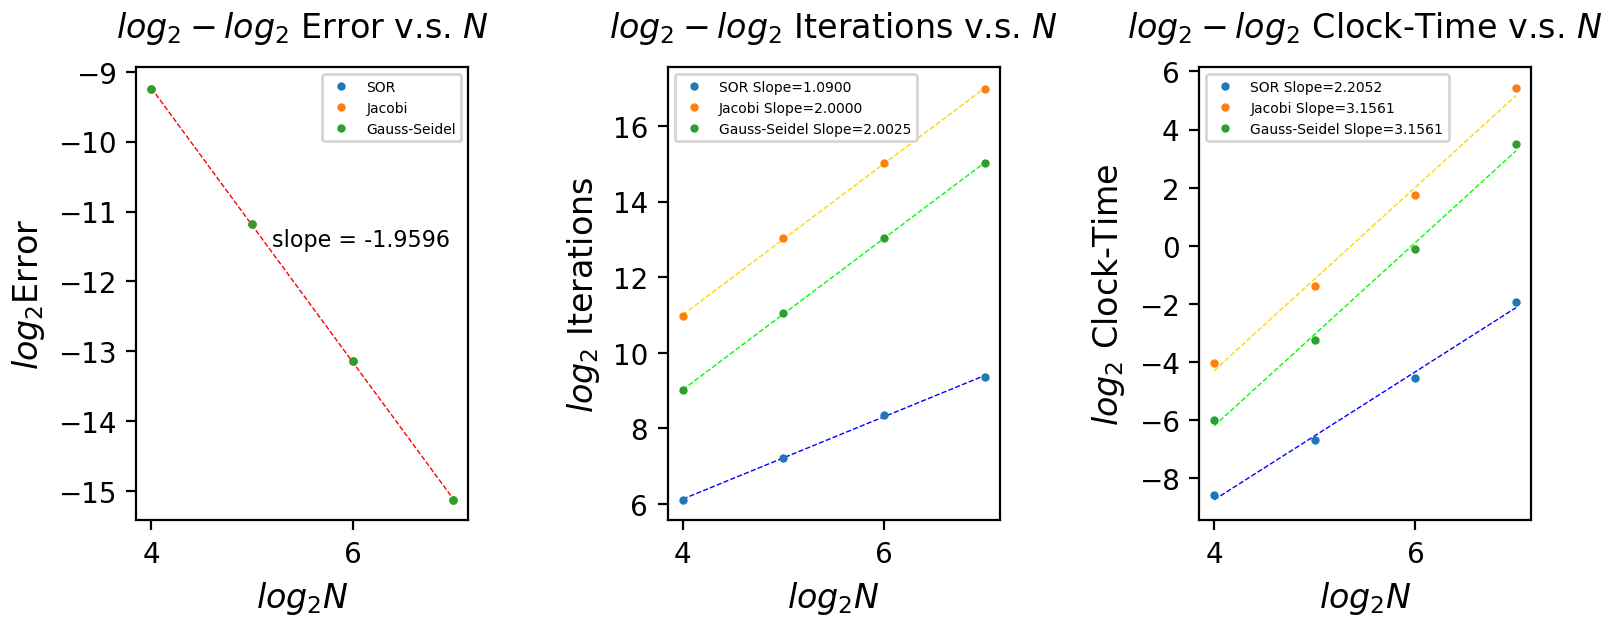
\includegraphics[width=19cm]{Problem_1_lattice_size_v.s.error_iterations_clock-time.png} %[]可選參數,控制圖片大小
%圖片說明
\caption{$log_2-log_2$ Error, Iterations and Clock-Time v.s. Lattice Size}
\end{figure}

\begin{figure}[htbp] %htbp 代表图片插入位置的设置
\centering %圖片置中
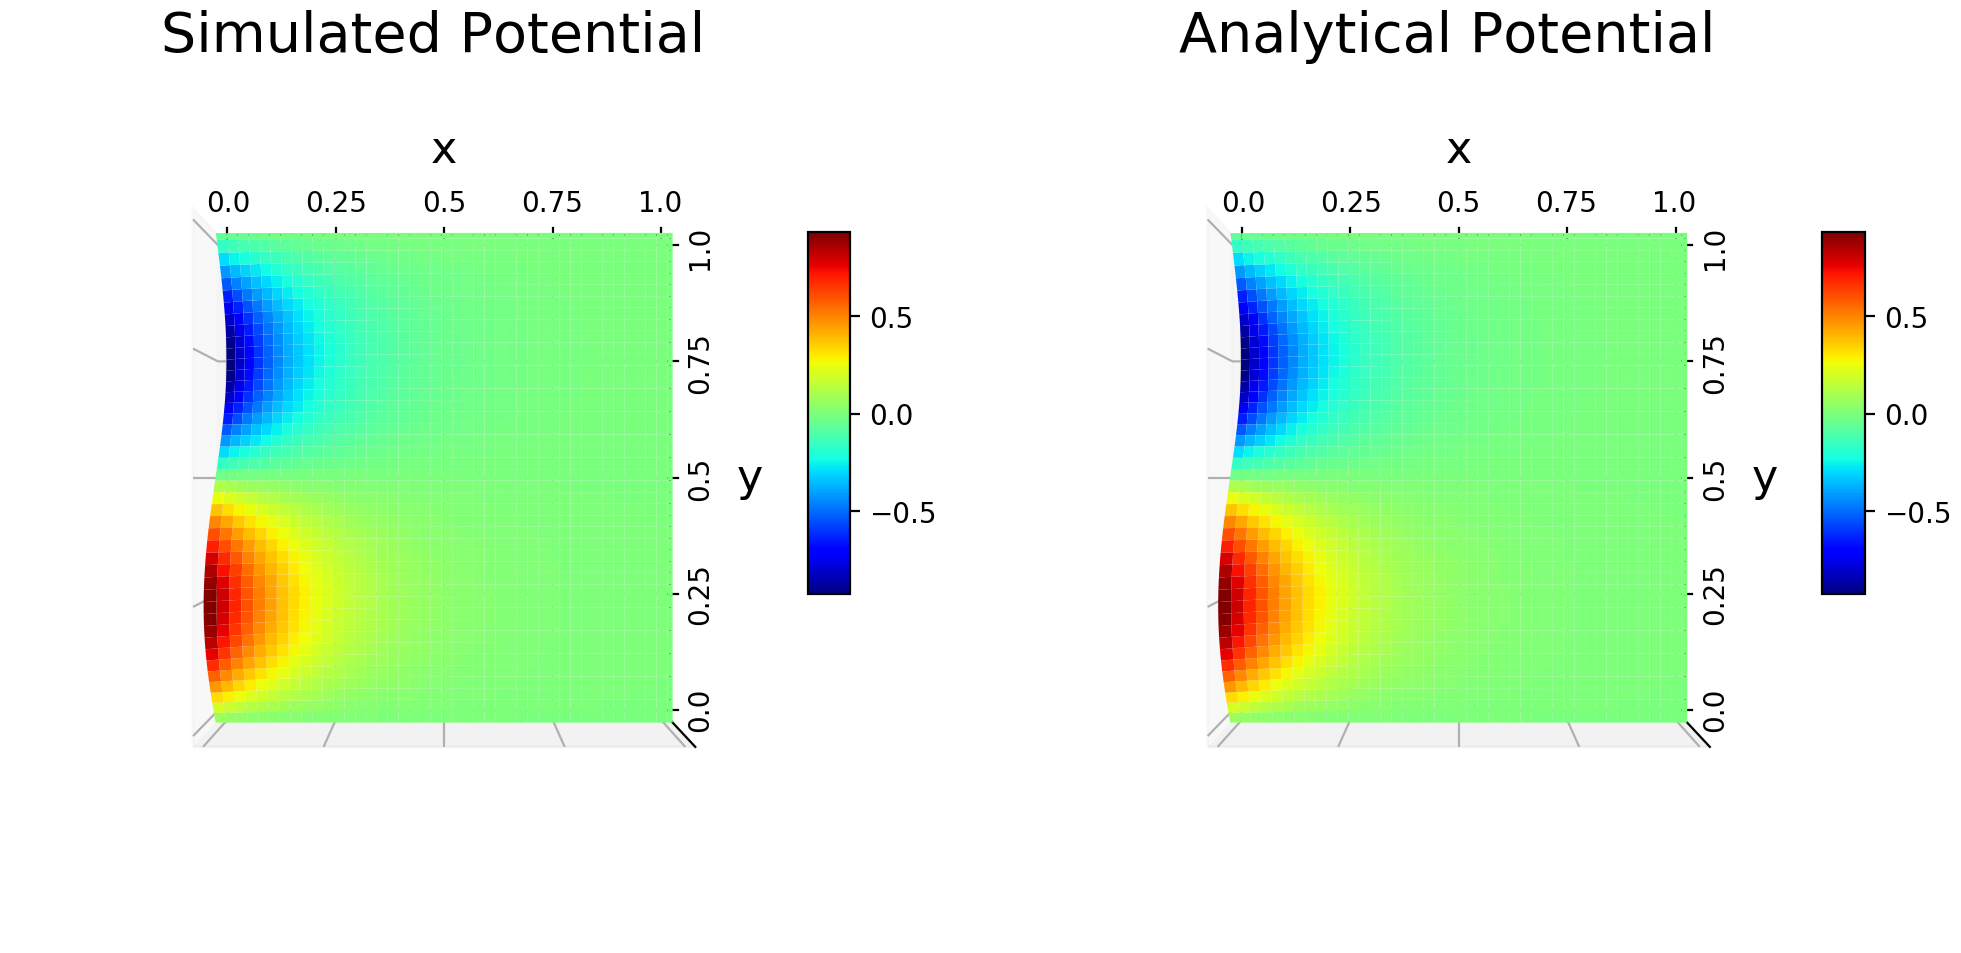
\includegraphics[width=19cm]{Problem_1_Simulated_v.s._Analytic_Potential_N=256_criteria=1.00000000e-21.png} %[]可選參數,控制圖片大小
%圖片說明
\caption{Simulated v.s. Analytic Field with $N=256$}
\end{figure}

\begin{figure}[htbp] %htbp 代表图片插入位置的设置
\centering %圖片置中
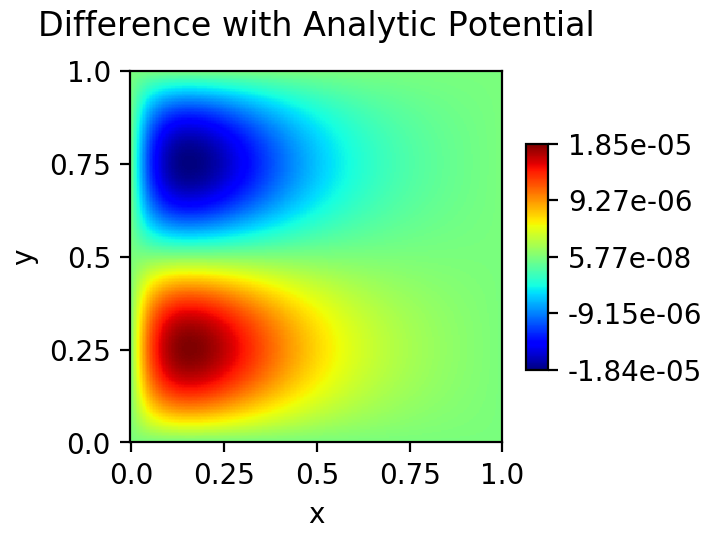
\includegraphics[width=13cm]{Problem_1_Simulated_v.s._Analytic_Potential_Difference_N=256_criteria=1.00000000e-21.png} %[]可選參數,控制圖片大小
%圖片說明
\caption{Difference between Simulated and Analytic Field with $N=256$}
\end{figure}

\end{large}

\newpage
\section*{Problem 2}
\begin{large}
Here we tested the sucessive over-relaxation scheme with $\omega$ varying from 0.25 to 1.99 with 0.01 interval, setting stopping criteria as $10^{-21}$. $\omega$ beyond 2.0 simply results in diverging field distribution, which serves as an upper bound. As the figure shows, the required iterations for convergence first decreases monotonically, and increases drastically after reaching a optimal value which is different for various lattice sites (specified in table 4). The optimal value is further fitted by
\begin{align*}
\omega = \frac{4}{2+\sqrt{4-4cos^2\frac{\pi}{N}}},
\end{align*}
which is shown in Fig 5.

 The curve-shape of total time is similar to that of total iterations: initially less time for higher $\omega$ to reach convergence, followed by a sharp increase after passing the optimal $\omega$. The only difference is that for a fixed $\omega$ (smaller than the optimal value), the iterations number for convergence scales by 4 while total clock time scales roughly by 8. 

\begin{figure}[htbp] %htbp 代表图片插入位置的设置
\centering %圖片置中
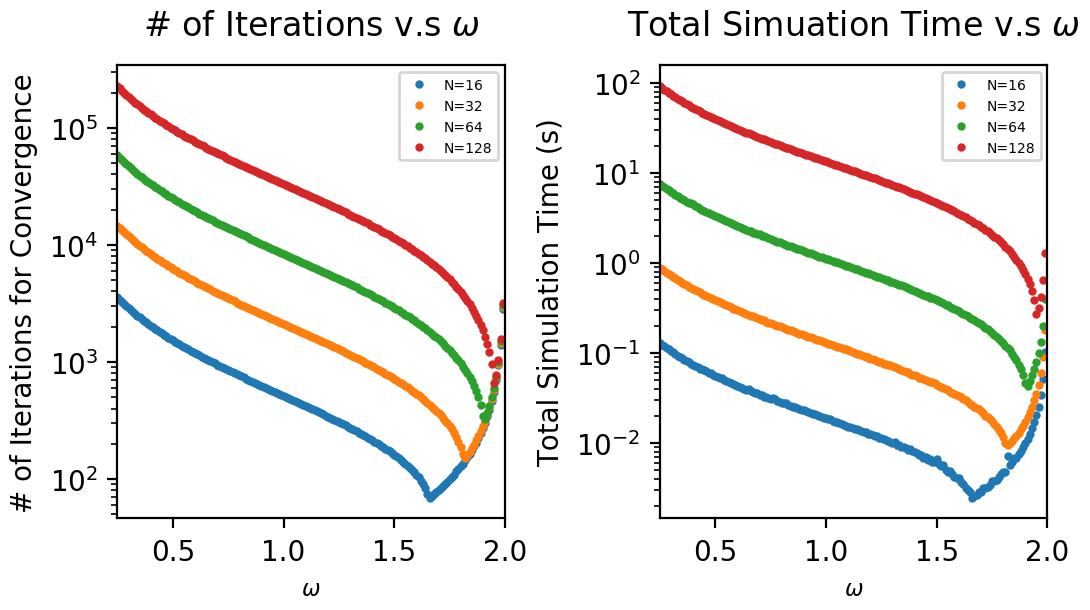
\includegraphics[width=15cm]{Problem_2_Optimal_omega_Fixed_Boundary.png} %[]可選參數,控制圖片大小
%圖片說明
\caption{Number of Iterations and Total Time v.s. $\omega$}
\end{figure}

\begin{table}[h]  %table 里面也可以嵌套tabular,只有tabular是不能加标题的
\centering  %表格居中
\begin{tabular}[t]{|c|c|c|c|}
\hline
Lattice size&Optimal $\omega$& Total Iterations\\
\hline
16&1.66&69\\
\hline
32&1.82&150\\
\hline
64&1.91&326\\
\hline
128& 1.95&661\\
\hline
\end{tabular}
\caption{Optimal $\omega$ of Different Lattice Size}  %表格标题
\end{table}

\begin{figure}[htbp] %htbp 代表图片插入位置的设置
\centering %圖片置中
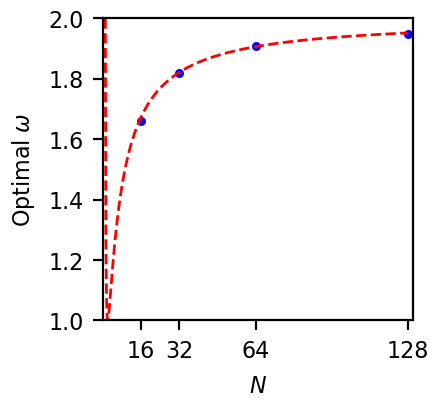
\includegraphics[width=7cm]{Problem_2_Optimal_omega_v.s._N_Fixed_Boundary.png} %[]可選參數,控制圖片大小
%圖片說明
\caption{Optimal $\omega$ Fitting}
\end{figure}

\newpage
Besides solving the Laplace equation, we also tried solving Poisson equation, where a unit charge is placed on the $([N/2], [N/2])$ site of a $N\times N$ lattice. The error for convergence is calculated by the difference of $\nabla^2 \phi$ and the Fourier transformed charge distribution. The fourier transform is utilized to obtain the "analytic" scalar field, with
\begin{align*}
\phi(\va{k})=\frac{1}{2}\frac{\Delta x^2\rho(\va{k})}{cos(k_x\Delta x)+cos(k_y\Delta x)-2}.
\end{align*}
Periodic boundary condition is imposed, along with extra condition that $\phi(0,0)=0$ to serves as reference point. 

Below we show how iterations and total time change with $\omega$, with stopping criteria $10^{-21}$. The curves are similar to that of scalar field without source, with the optimal value given in table 5. The field is shifted by $\phi(0,0)$ after the simulation converges. We can see the number of iterations as well as the total time is even less than that of scalar field without source. I guess this is because we did not impose any bounday condition, so the information on one side does not need to propagate all the way to the opposite side; the field can reach equilibrium once the field induced by the charge situated at center propagtes to the boundaries, which should spend less time.

\begin{table}[h]  %table 里面也可以嵌套tabular,只有tabular是不能加标题的
\centering  %表格居中
\begin{tabular}[t]{|c|c|c|c|}
\hline
Lattice size&Optimal $\omega$& Total Iterations\\
\hline
16&1.58&51\\
\hline
32&1.76&107\\
\hline
64&1.88&226\\
\hline
128& 1.94&481\\
\hline
\end{tabular}
\caption{Optimal $\omega$ of Different Lattice Size for Scalar Field with Source (Periodic)}  %表格标题
\end{table}

We further checked our guess using the same problem but this time specified the field strength on the boundaries, whose optimal $\omega$ is listed in table 6, and is very close to scalar field without source. The iterations number does increase for all lattice size as expected. In Fig. 7, the curve of $N=128$ with $\omega$ above 1.95 is truncated bcause it cannot hit the stopping criteria.

\begin{table}[h]  %table 里面也可以嵌套tabular,只有tabular是不能加标题的
\centering  %表格居中
\begin{tabular}[t]{|c|c|c|c|}
\hline
Lattice size&Optimal $\omega$& Total Iterations\\
\hline
16&1.66&73\\
\hline
32&1.82&153\\
\hline
64&1.91&338\\
\hline
128& 1.94&1289\\
\hline
\end{tabular}
\caption{Optimal $\omega$ of Different Lattice Size for Scalar Field with Source (Periodic)}  %表格标题
\end{table}

\begin{figure}[htbp] %htbp 代表图片插入位置的设置
\centering %圖片置中
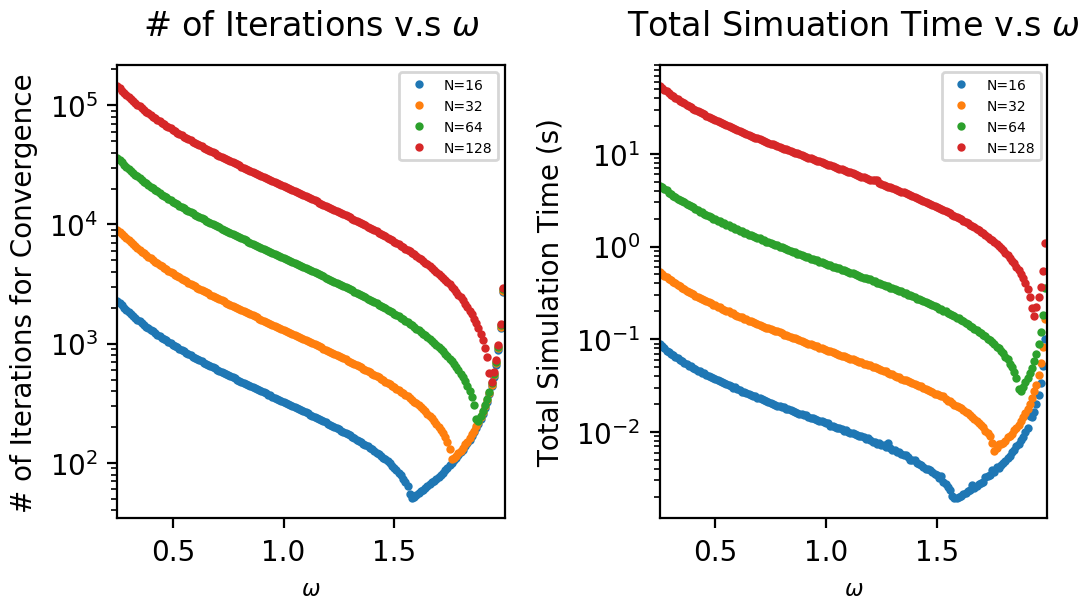
\includegraphics[width=15cm]{Problem_2_Optimal_omega_with_Charge_Periodic.png} %[]可選參數,控制圖片大小
%圖片說明
\caption{Number of Iterations and Total Time v.s. $\omega$ for Scalar Field with Source (Periodic)}
\end{figure}

\begin{figure}[htbp] %htbp 代表图片插入位置的设置
\centering %圖片置中
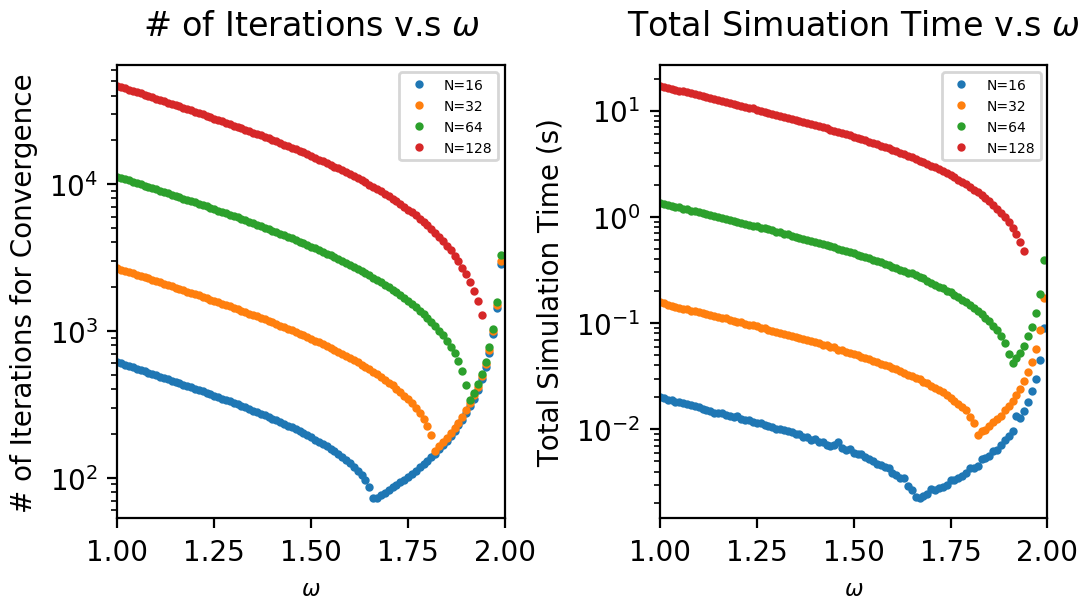
\includegraphics[width=15cm]{Problem_2_Optimal_omega_with_Charge_Fixed_Boundary.png} %[]可選參數,控制圖片大小
%圖片說明
\caption{Number of Iterations and Total Time v.s. $\omega$ for Scalar Field with Source (Fixed Boundary)}
\end{figure}

\end{large}
\newpage
\section*{Problem 3}
\begin{large}
For the results of iterations and clock-time for scalar field without source for Jacobi, Gauss-Seidel and sucessive over-relaxation, please refer to Fig. 1 and discussion in Problem 1. 

Here we show the lattice size dependence of iterations number and total time for scalar field with source (stopping criteria set as $8\times10^{-20}$ since Jacobi with 128 lattice size cannot converge if criteria is set as $10^{-21}$). The iterations needed for convergence scale up roughly as $2^{2.3}=4.92$ for Jacobi, $2^{2}$ for Gauss-Seidel and $2^{1.08}=2.11$ for successive over-relaxation when lattice size $N$ doubled, suggesting that successive over-relaxation is still the most efficient one, Gauss-Seidel is the second, and Jacobi is the worst, which can be verified by checking thenumber of iterations and total time.

For total time, the scaling expontent is 3.47 for Jacobi, 3.08 for Gauss-Seidel and 2.15 for successive over-relaxation, i.e., the time increases by a factor of 11.08, 8.46 and 4.44 for each scheme when lattic size doubled, seems to indicate single iteration takes more time if lattice is large (if iteration takes same amount of time irrelevent of lattice size, total time should proportional to iteration number), whose growing rate roughly $\propto N$.  

Field distribution with fixed boundary condition is also simulated, which shows the total iterations scale up as $2^{2.08}=4.23$ for Jacobi and Gauss-Seidel, $2^{1.33}=2.51$ for successive over-relaxation when $N$ doubled. The corresponding scaling factors for total time are $2^{3.24}$ for Jacobi, $2^{3.21}$ for Gauss-Seidel and $2^{2.46}$ for successive over-relaxation, similar to that of PBC case. We notice that Jacobi method converges quicker than PBC case, while Gauss-Seidel and successive over-relaxation beome slower.

The field distribution and the difference with analytic solution is also attached (for periodic boundary condition), from which we can see good agreement with analytic solution.
\begin{figure}[htbp] %htbp 代表图片插入位置的设置
\centering %圖片置中
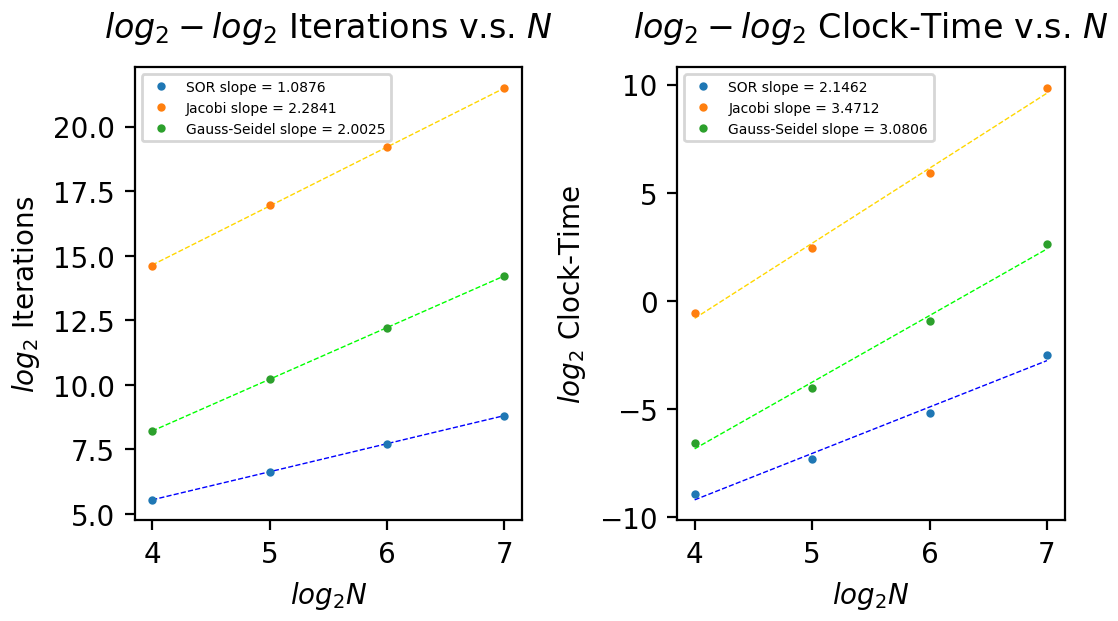
\includegraphics[width=15cm]{Problem_3_lattice_size_v.s.iterations_clock-time_with_Charge_Periodic.png} %[]可選參數,控制圖片大小
%圖片說明
\caption{$log_2-log_2$ Iterations and Clock-Time v.s. Lattice Size for Scalar Field with Source (Periodic)}
\end{figure}

\begin{figure}[htbp] %htbp 代表图片插入位置的设置
\centering %圖片置中
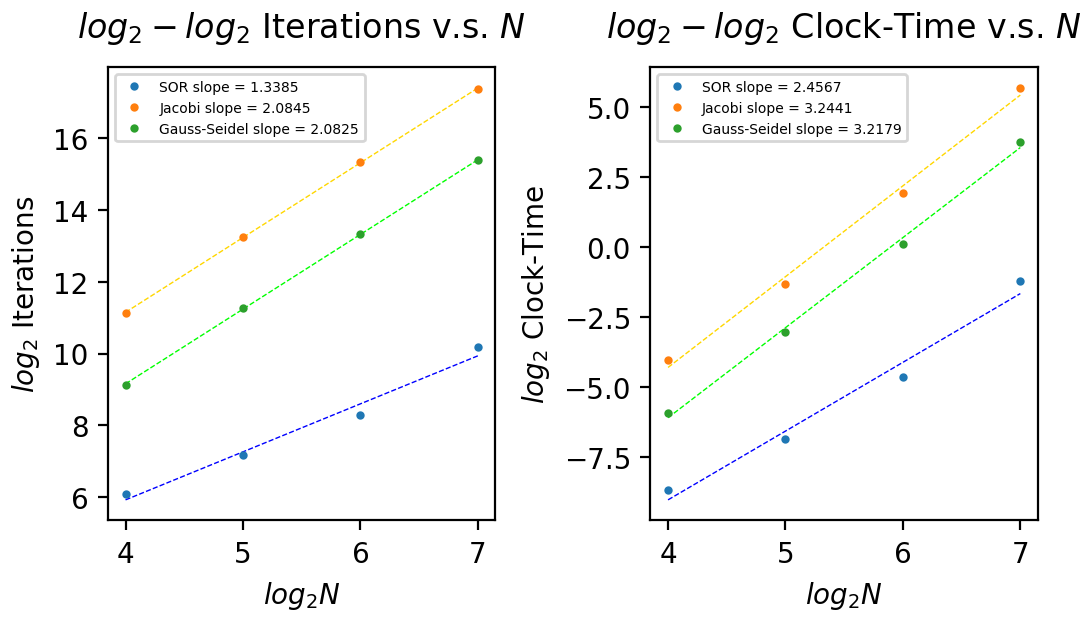
\includegraphics[width=15cm]{Problem_3_lattice_size_v.s.iterations_clock-time_with_Charge_Fixed_Boundary.png} %[]可選參數,控制圖片大小
%圖片說明
\caption{$log_2-log_2$ Iterations and Clock-Time v.s. Lattice Size for Scalar Field with Source (Fixed Boundary)}
\end{figure}

\begin{figure}[htbp] %htbp 代表图片插入位置的设置
\centering %圖片置中
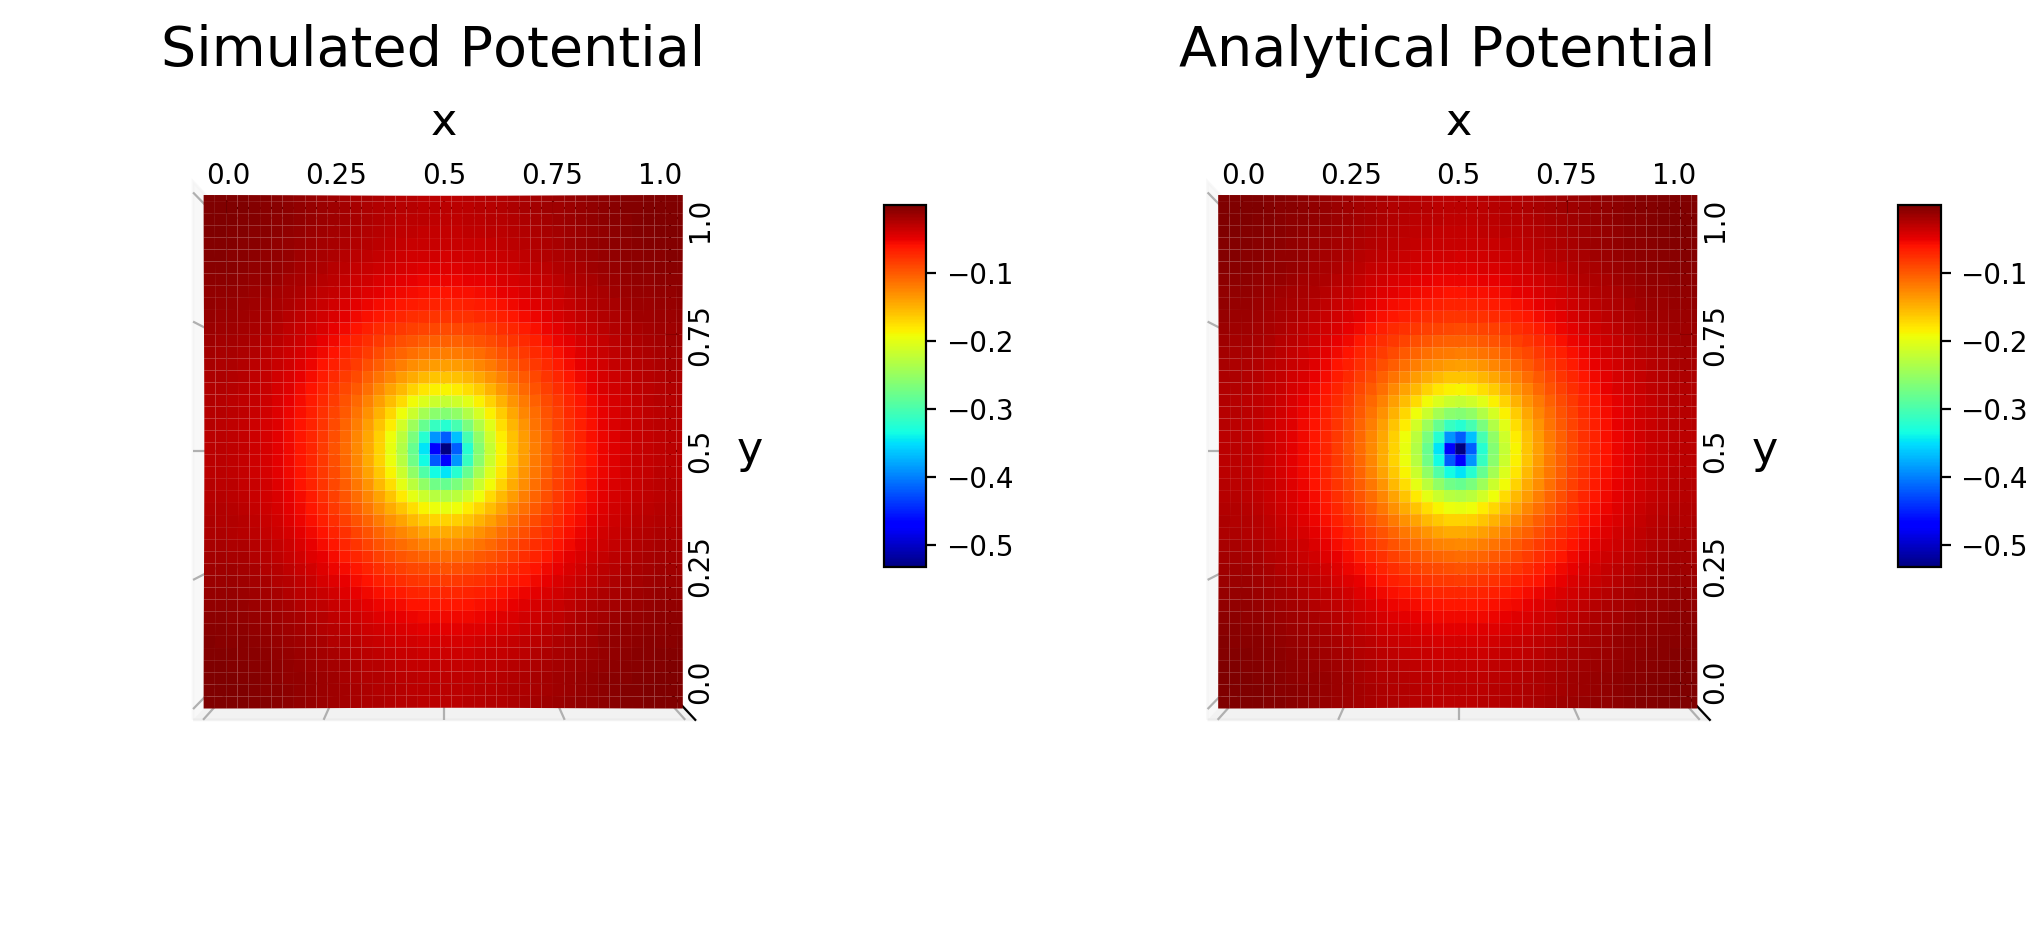
\includegraphics[width=15cm]{Problem_3_Simulated_v.s._Analytic_Potential_N=256_criteria=1.00000000e-21_with_Charge_Periodic.png} %[]可選參數,控制圖片大小
%圖片說明
\caption{Simulated v.s. Analytic Field with $N=256$ for Scalar Field with Source (Periodic)}
\end{figure}

\begin{figure}[htbp] %htbp 代表图片插入位置的设置
\centering %圖片置中
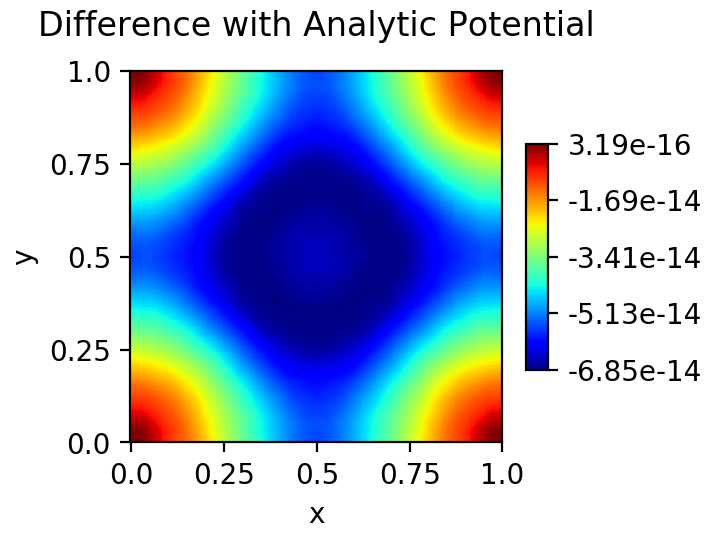
\includegraphics[width=13cm]{Problem_3_Simulated_v.s._Analytic_Potential_Difference_N=256_criteria=1.00000000e-21_with_Charge_Periodic.png} %[]可選參數,控制圖片大小
%圖片說明
\caption{Difference between Simulated and Analytic Field with $N=256$ for Scalar Field with Source (Periodic)}
\end{figure}

\end{large}
\end{document}
